\chapter{Proposition de modèle de représentation des chaînes de caractères et contributions}\label{solution_chap}

Les chaînes de caractères sont des structures de données primordiales pour un langage de programmation.
Tous les langages proposent un modèle, chacun avec ses avantages et ses inconvénients.
Certains privilégient la facilité d'utilisation et la parallélisation via des chaînes immutables,
d'autres privilégient la rapidité via des chaînes mutables.
Au niveau de la structure de données, le tableau de caractères est la structure la plus fréquente
dans les langages impératifs et à objets.
Cependant, les problèmes de la structure, détaillés en section~\ref{state_flatstr_prez}, en
ce qui concerne le passage à l'échelle nous font demander s'il n'est
pas possible de l'améliorer, tout en gardant l'utilisation aussi simple que possible du point
de vue des utilisateurs du langage.

Ce chapitre présente le modèle des chaînes de caractères en Nit, 
les modifications que nous avons apporté à la bibliothèque standard, pourquoi nous avons pris
ces décisions et quels sont les travaux restants.

\section{Ancien modèle}

\subsection{Les chaînes sous forme de tableau}

Au début de ce travail, les chaînes de Nit étaient uniquement des tableaux de caractères.
La définition de caractère selon le langage était calquée sur celle de C: un caractère Nit
était un \texttt{char} C, c'est à dire un octet.
Les manipulations étaient orientées octet et le contenu d'une chaîne n'était pas partagé,
la production d'une sous-chaîne de caractères entraînait l'allocation et la copie partielle du
contenu de la chaîne d'origine.
Les chaînes de caractères étaient des enveloppes autour d'un \texttt{char*} natif: \texttt{NativeString}
(voir figure~\ref{oldmodel}).

Il existait deux alternatives dans la construction des chaînes de caractères:

\begin{enumerate}
	\item\texttt{String}: chaîne de caractères immutable.
	\item\texttt{Buffer}: chaîne de caractères mutable, notamment utilisée pour la concaténation et les modifications efficaces.
\end{enumerate}

\begin{figure}
	\caption{Ancien mod\`{e}le des chaînes de Nit}
	\label{oldmodel}
	\centering
	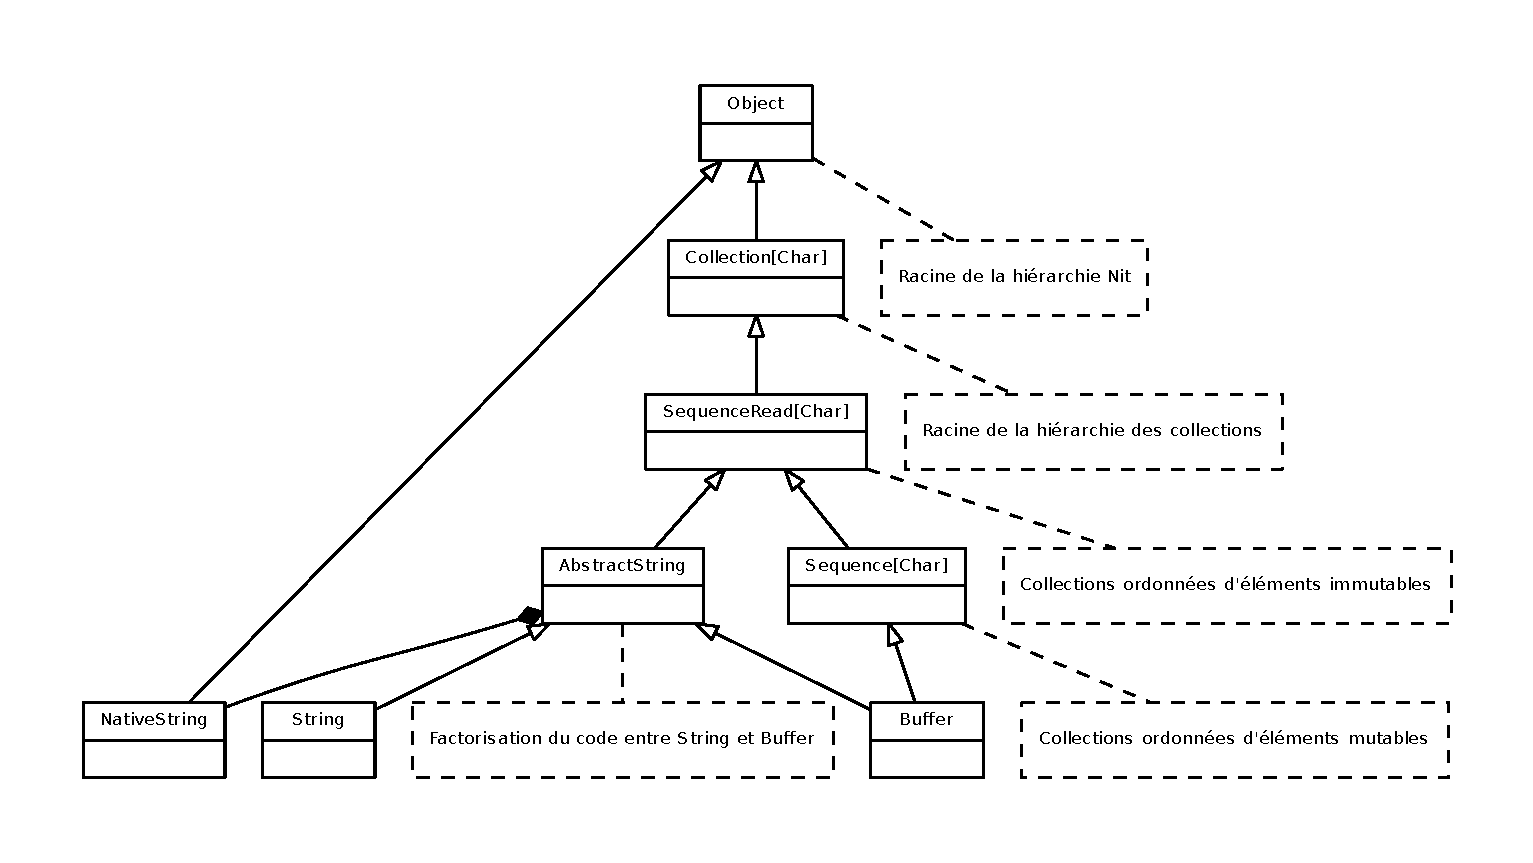
\includegraphics[angle=90, scale=0.75]{figures/old_model.pdf}
\end{figure}

Malgré le non-support d'un codage multilingue, l'ancien modèle possédait des avantages certains:

\begin{enumerate}
	\item Les accès à un caractère étaient effectués en temps constant.
	\item La structure en \texttt{char*} permettaient un passage facile et peu coûteux vers les morceaux de code C.
	\item Le modèle était simple à comprendre.
\end{enumerate}

Cependant, malgré ces avantages, il possèdait toutes les limitations dûes aux chaînes plates,
qui malheureusement ne peuvent être résolues simplement en optimisant les opérations effectuées sur ces
dernières.

\begin{enumerate}
	\item Pas de résistance face aux traitements sur de longues chaînes.
	\item Cas dégénératifs lors de concaténations de grandes chaînes.
\end{enumerate}

\subsection{Codage}\label{codage_ancien}

Les chaînes de caractères en Nit étaient anciennement de simples séquences d'octets, aucune
information de codage n'était disponible.
L'ensemble des opérations disponibles se basaient sur les sémantiques de l'ASCII, et tous les caractères
en dehors de cette zone étaient ignorés, menant parfois à des résultats erronés du point de vue de
l'utilisateur.

En effet, un simple programme comme celui-ci:

\begin{verbatim}
var s = "être"
for c in s.chars do printn "{c}-"
\end{verbatim}

Produisait le résultat erroné: \texttt{{\fontspec{DejaVu Sans}�}-{\fontspec{DejaVu Sans}�}-t-r-e-}

Dans la mesure où ASCII n'est pas le seul codage capable de représenter des chaînes de caractères en
utilisant l'octet comme codet, aucune manipulation n'était véritablement sûre et du texte codé dans un
codage possédant une représentation similaire (KOI-8, GOST-10859, etc.) risquait d'être corrompu.

\section{Nouveau modèle}

\subsection{Codage}

Du fait des limitations présentées en~\ref{codage_ancien}, nous avons changé les chaînes Nit
en séquences de points de code, codées en UTF-8.
Il est désormais possible d'accéder indépendamment aux octets ou aux points de code.

Le support de ces opérations nous permet, sur le morceau de code développé en~\ref{codage_ancien},
de produire le résultat attendu communément: \texttt{ê-t-r-e-}

Les chaînes sont également nettoyées lors du passage d'un objet binaire à une chaîne de caractères de façon
à ce qu'elle ne contienne que des séquences UTF-8 valides.
Par \og nettoyées \fg{}, nous entendons que les séquences UTF-8 invalides sont remplacées par le
caractère de remplacement Unicode {\fontspec{DejaVu Sans}�} (U+FFFD).
Une séquence UTF-8 invalide peut avoir plusieurs formes, il peut s'agir de séquences incomplètes,
d'octets invalides dans un point de code, ou de séquences trop longues.
Par exemple, une séquence \texttt{0xC0 0xAF} est considérée comme trop longue pour représenter
le caractère \texttt{/}, et sa véritable valeur devrait être \texttt{0x2F}.

Cette opération est obligatoire selon le standard Unicode pour assurer une bonne compatiblité
avec les séquences de texte en UTF-8.
Les bibliothèques n'effectuant pas ce type de manipulations s'exposent potentiellement à des soucis de sécurité.
Une vulnérabilité de ce style était présente en PHP par exemple via la fonction \texttt{$mysql\_real\_escape\_string$}.
En injectant une séquence trop longue, la fonction de validation ne nettoie pas le \texttt{'}, et
le caractère qui aurait du être rejeté est accepté.
Cette faille permettait à un tiers malveillant d'injecter du code SQL arbitraire dans une requête.

\subsection{Cordes}

En Nit, nous utilisons les cordes en conjonction des chaînes plates pour plusieurs
raisons.

Le fait qu'aussi bien en UTF-8 qu'en UTF-16, l'accès aux caractères s'effectue de façon linéaire\footnote{Note:
Des langages comme Java et C\# proposent un accès en temps constant en UTF-16, mais l'accès est
non-sûr dès lors qu'un caractère hors-BMP est présent.}
permet aux cordes de mitiger l'utilisation de ces codages dans des chaînes de grande taille en réduisant
l'accès à une complexité temporelle de O(log(n)) pour la sous-chaîne contenant le caractère visé,
puis en O(n) sur une feuille\footnote{Une feuille est une chaîne plate présente à l'extrêmité d'une corde.}.
Cette complexité suppose que la corde sur laquelle l'opération d'accès est effectuée est équilibrée.
En termes d'utilisation mémoire, les cordes sont également avantageuses du fait de la séparation des
chaînes en parties de faible taille.
Le sous-chaînage et des opérations de modification de contenu par exemple permettent de limiter les réallocations
dans les cas où seulement une partie de la chaîne d'origine doit être ré-allouée au lieu de l'ensemble de
la chaîne (i.e. trim, ou seulement la première et la dernière feuille nécéssitent une ré-allocation).

\subsection{L'implémentation en Nit}

Du fait des faiblesses de l'ancien modèle, notamment en termes de passage à l'échelle, nous
proposons un nouveau modèle original pour les utilisateurs du langage, que nous avons
implémenté en Nit.
Il s'articule autour d'une classe abstraite de manipulation du texte: \texttt{Text}.
Un autre changement majeur de ce nouveau modèle en termes d'API vient également de la différenciation
entre les manipulations orientées octet et les manipulations orientées texte.

Deux sous-classes de \texttt{Text} sont exposées: \texttt{String}, pour des chaînes de caractères immutables, et \texttt{Buffer}
pour les chaînes de caractères mutables.
En plus de la différence entre mutable et immutable, deux sous-classes de \texttt{Text} sont
introduites: \texttt{FlatText} et \texttt{Rope}.

\texttt{FlatText} définit la base des chaînes de caractères plates, ce sont des enveloppes autour de tableaux d'octets C.
\texttt{Rope} quant à lui est une structure sous forme de corde, deux implémentations sont disponibles: \texttt{Concat}, une
corde immutable, et \texttt{RopeBuffer}, une version mutable de corde.
Notons que ce dernier est expérimental et était peu performant au moment de rédiger ces lignes.
Une vue d'ensemble de ce modèle est présentée dans la figure~\ref{newmodel}.

Nous proposons de changer de façon transparente au programmeur la représentation interne des
chaînes de caractères pour éviter les cas dégéneratifs exposés par les chaînes plates.
Pour éviter les allocations trop nombreuses et limiter la taille des allocations, qui
deviennent coûteuses passées un certain seuil,
la concaténation de chaînes de caractères est implementée
de façon à produire un noeud de concatenation au lieu de ré-allouer une nouvelle
chaîne plate et d'effectuer une copie de contenu.

\begin{Verbatim}[obeytabs,tabsize=4]
class Text
	fun +(o: Text) do
		var result: String
		if byte_length + o.byte_length > concatenation_seuil then
			result = new Concat(to_s, o.to_s)
		else
			var new_arr = malloc(byte_length + o.byte_length)
			copy_content(new_arr, byte_length, 0)
			o.copy_content(new_arr, o.byte_length, byte_length)
			result = new FlatString(new_arr)
		end
		return result
	end
end
\end{Verbatim}

Cette approche permet également un accès en temps logarithmique au lieu de linéaire
à un caractère abritraire d'une chaîne de caractères.
Si cette faculté est intéressante, elle reste néanmoins anectodique dans la mesure où il s'agit d'un cas de
figure assez rare, les caractères d'une chaîne étant le plus souvent accédés de façon itérative.

Lors de l'introduction d'Unicode dans Nit, il nous est apparu important de faire une distinction claire entre les API
orientées caractères, où un caractère référence le graphème ou le point de code, et les
API orientées sur leur représentation sous-jacente, dans notre cas l'octet.
Il s'agit d'une différence que les implémentations existantes font rarement, et jusqu'à aujourd'hui, parmi les
langages populaires, seuls Perl6, Swift ou Elixir font une réelle distinction entre ces entités.

Pour permettre aux utilisateurs du langage d'accéder au besoin à la représentation sous-jacente,
toutes les représentations de chaînes de caractères disponibles possèdent un systeme de vue sur les différentes
entités du contenu d'une chaîne de caractères: \texttt{Byte} et \texttt{Char}.
Dans le futur, nous souhaitons également proposer une vue orientée \texttt{Graphème} pour accéder au contenu
d'une chaîne de caractères, à l'instar de ce que proposent Perl6 ou Swift.
Présentement, les opérations d'accès par défaut d'une chaîne opèrent au niveau du point de code.
Ce choix est arbitraire, un travail futur permettrait de déterminer si l'accès devrait
se faire au niveau du graphème par défaut, ou non.

\begin{figure}
	\caption{Nouveau mod\`{e}le des chaînes de Nit}
	\label{newmodel}
	\centering
	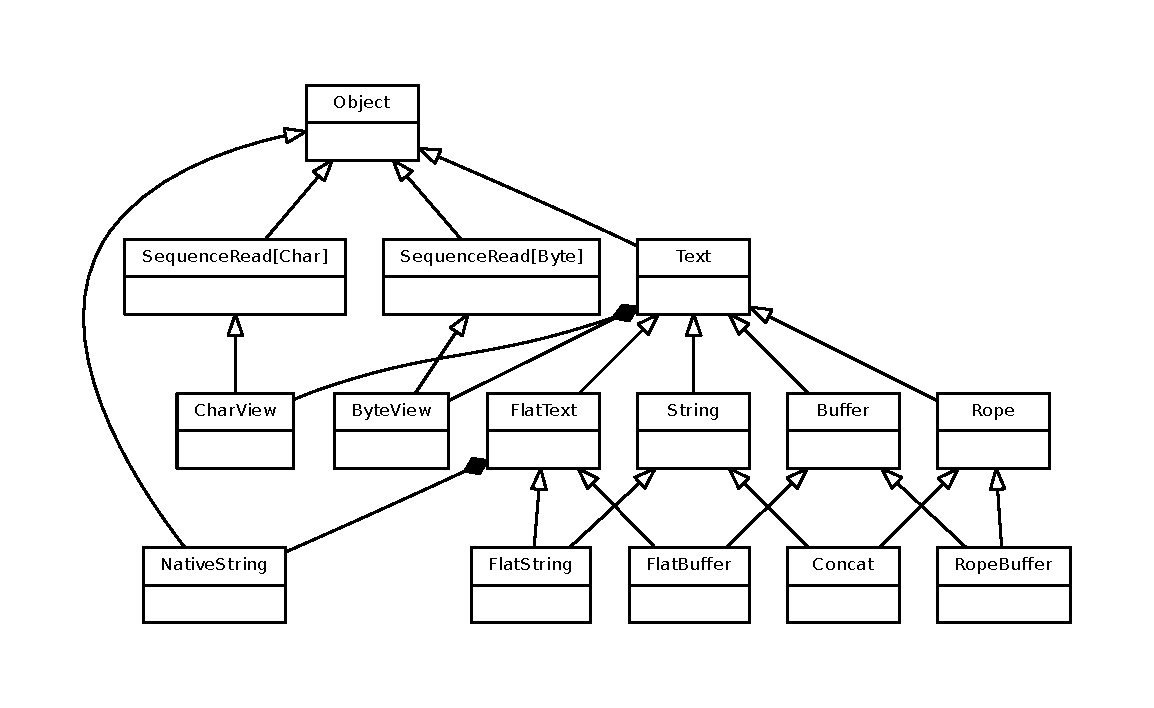
\includegraphics[angle=90]{figures/new_model.pdf}
\end{figure}

La solution que nous présentons expose un modèle complexe à l'implémentation, mais simple à l'utilisation.
Les classes \texttt{FlatString}, \texttt{FlatBuffer}, \texttt{Concat} et \texttt{RopeBuffer} continuent
à être exposées à l'utilisateur pour des raisons de performances dans des cas particuliers.
Cependant, ce dernier continue à interagir avec des chaînes de caractères par le biais des classes abstraites
\texttt{String} et \texttt{Buffer}, ce qui permet de garder une API simple, peu importe la complexité
de la structure sous-jacente.
Notons que l'implémentation de ce modèle a largement été simplifié par le support de l'héritage
multiple en Nit.
S'il est possible d'implémenter un modèle similaire en Java ou dans un autre langage, la réalisation
sera plus complexe et le modèle en découlant comportera plus d'interfaces.

\section{Bibliothèque}

Une première partie du travail en termes d'API consistait à désolidariser les chaînes de caractères
du bloc des collections.
Nous avons pris cette décision du fait de la non-applicabilité de certains services
à des structures comme les chaînes de caractères.

Par exemple, le service \texttt{join} est peu utile dans le cadre d'une chaîne de caractères et avait pour effet
de joindre un motif entre chaque caractère.
D'autres services comme \texttt{sort} par exemple ont peu de sens quand utilisés sur une chaîne,
où le résultat serait d'avoir les caractères triés par ordre lexicographique.

Une partie du travail s'est focalisé sur l'intégration du bloc des cordes.
Nous avons essayé plusieurs alternatives avant de garder l'implémentation actuelle.
Une première était basée sur l'implémentation de SGI Rope, disponible aujourd'hui via les extensions
STL C++ de GNU GCC\footnote{Code disponible à \url{https://gcc.gnu.org/onlinedocs/gcc-4.6.3/libstdc++/api/a01015_source.html}.}.
Cependant, les structures présentées par cette implémentation étaient lourdes de par la création de noeuds
feuille.
Cela nous a contraint à abandonner l'ancien code en faveur de l'actuel, inspiré
de l'implémentation de Boehm, disponible dans le ramasse-miettes du même
nom\footnote{Paquet disponible à \url{https://github.com/ivmai/bdwgc/tree/master/cord}.}.
On notera que les cordes d'SGI comportent deux types de noeud spéciaux en plus de ceux exposés par les notres:

\begin{enumerate}
	\item Noeud fonction: un type de noeud contenant deux références, un vers la corde, et un vers une fonction.
		Ils sont utilisés lors de traitements paresseux sur les cordes. Nit ne permettant pas de représenter et
		d'invoquer une fonction arbitrairement, ils sont laissés de côté dans notre implémentation.
	\item Noeud de sous-chaînage: ces noeuds permettent de créer en temps constant une sous-chaîne en fonctionnant
		d'une façon similaire à la fonction \texttt{substring} de Nit.
		Ils contiennent un pointeur vers une corde, ainsi qu'un index de départ de la sous-chaîne dans cette corde.
		Leur principale raison d'être est leur compatibilité avec les noeuds fonction, afin
		d'effectuer les calculs nécessaires à la production de la sous-chaîne de façon paresseuse.
\end{enumerate}

Une autre partie du travail effectué a été sur l'intégration d'Unicode à la bibliothèque standard.
Il a fallu changer la sémantique et le type associé dans le C généré de \texttt{Char}, dans la mesure
où un caractère a évolué d'octet à point de code.
Ce changement a posé un nombre conséquent de problèmes:

\begin{enumerate}
	\item Clients brisés: certains clients se servaient de chaînes de caractères comme d'un tableau d'octets et se basaient sur l'équivalence entre les chaînes et ces mêmes tableaux; en changeant le type de Char, le code qui dépendait de cette sémantique s'est retrouvé brisé.
	\item Problèmes d'amorçage: Nit possèdant un compilateur autogène, l'ensemble des modifications de la bibliothèque ont des impacts sur la façon dont le compilateur se compile lui-même. En changeant un type primitif, certaines signatures et opérations provoquaient des erreurs dans le C généré par une ancienne version du compilateur, empêchant par ce fait le compilateur de fonctionner.
	\item Problèmes avec les morceaux de code externe: une partie de la bibliothèque de Nit est implémentée directement en C via un mécanisme de FFI\footnote{Foreign Function Interface: Façon d'appeler du code externe depuis du code Nit et vice-versa}~\cite{xymus_memoire}.
		Une partie de ces morceaux de code dépendaient directement de la correspondance entre \texttt{Char} Nit et
		\texttt{char} C.
		En changeant la définition de \texttt{Char} côté Nit, ces utilisations en C doivent changer également et pour
		un certain nombre, le changement ne se limite pas à un simple cast.
\end{enumerate}

Au-delà du changement de sémantique dans les types primitifs,
nous avons changé les opérations de la bibliothèque standard.
Principalement en termes de performance, où des opérations comme
l'accès indexé, qui s'effectuait en temps constant, ont évolué pour s'effectuer en temps linéaire.
Les impacts de ce changement nous ont forcé à inclure un système de cache aux chaînes, de façon à limiter cet impact.
Cependant, il reste des cas où Unicode nous empêche de préserver les mêmes performances.
Un de ces cas est la modification.
En effet, lorsque l'on souhaite remplacer un caractère dans un \texttt{buffer}, il se peut que l'opération doive
s'effectuer en temps linéaire.
Il s'agit là d'un des problèmes majeurs des codages à longueur variable comme UTF-8 ou UTF-16, où le remplacement
d'un caractère peut avoir comme effet de déplacer toutes les données du buffer pour combler ou récupérer
de l'espace.

Par exemple, dans ce morceau de code:

\begin{verbatim}
var b = new Buffer.from("Être")
b[0] = 'E'
\end{verbatim}

Le remplacement de la lettre 'Ê' par 'E' en UTF-8 force le déplacement des caractères suivants de 1 octet vers la
gauche.

Un dernier changement, qui lui aussi a eu des implications sur certains clients, est le nettoyage des objets binaires
lors de leur passage à une chaîne Unicode.
Les bogues liés à ces comportements-là sont bien souvent liés à des programmes similaires à ceux ayant eu des problèmes
lors du changement de sémantique de \texttt{Char}.
En effet, en modifiant le contenu du tableau de caractères sous-jacent à une chaîne, les programmes se servant de
chaînes de caractères comme espace temporaire de stockage des données binaires ont fait face à des corruptions des
données, résultant en des bogues difficiles à tracer pour les personnes non familières avec Unicode.

Ce problème a nécessité l'introduction de nouveaux types dans la bibliothèque standard:

\begin{enumerate}
	\item \texttt{Byte}: Un octet, représenté en Nit. Il s'agit d'un nouveau type primitif, visant
		à remplacer l'ancienne représentation de \texttt{Char}. Les opérations sur les \texttt{NativeString}
		ont toutes évolué pour supporter ce type.
	\item \texttt{Bytes}: Une collection d'octets mutable sous forme plate. Elles peuvent être utilisées
		à la place des anciennes \texttt{String} pour préserver la sémantique orientée octet de ces
		structures dans les cas où le texte n'est pas une priorité. Il est à noter que la conversion
		d'une chaîne de caractères vers un \texttt{Bytes} et vice-versa quand possible, 
		est effectuée via un mécanisme de \textit{copy-on-write}
		de façon à limiter l'impact de la transformation d'une représentation vers l'autre.
\end{enumerate}

En plus des contributions mentionnées plus haut, une preuve de concept d'internationalisation semi-automatique
a été intégrée à la suite d'outils Nit.
Elle a été implémentée sous la forme d'une annotation de module, qui une fois utilisée externalise les chaînes
littérales présentes dans un fichier source dans un fichier \texttt{po}, pour utilisation avec GNU \texttt{gettext}
et remplace leurs utilisations par un appel à \texttt{gettext} pour récupérer la chaîne traduite dans la locale
de l'utilisateur si disponible.
Il s'agit d'une façon standard de faire pour les applications sous Linux.
Il est possible via des modifications mineures de supporter d'autres systèmes d'internationalisation pour d'autres
plateformes, comme le fichier \texttt{R.java}
\footnote{Technique standard en Android pour externaliser des chaînes de caractères littérales à des fins d'internationalisation.}
pour Android par exemple.

\section{Micro-optimisations}

Les changements structurels et de codage nous ont forcé à profiter des attributs physiques de la machine pour
accélérer les opérations fondamentales des chaînes.
Une grande partie de ce travail a été dédié à la micro-optimisation, à l'étude du C et de l'assembleur généré,
ainsi qu'aux caractéristiques physiques des machines sur lesquelles les programmes Nit sont exécutés.
Parmi les optimisations que nous avons implémentées, nous pouvons en citer trois majeures.

\subsection{Accès multiple}

Une façon d'accélérer le parcours des chaînes de caractères est de pré-chercher plusieurs
caractères à la fois et d'effectuer des opérations sur eux. Nous nous servons de cette astuce pour quadrupler la vitesse
de parcours dans des chaînes en ASCII. Il est à noter que cette optimisation peut être améliorée en prenant en compte les
propriétés de différentes architectures. Par exemple, sur un processeur 64-bits, nous pourrions pré-charger 8 caractères
sans surcoût notable par exemple.

\subsection{Caches}

Pour accélérer les opérations courantes sur les chaînes, nous avons mis en place plusieurs systèmes
de cache, aussi bien dans les chaînes plates, que dans les cordes. Dans ces dernières, ils nous permettent de court-circuiter
le parcours de la corde et d'aller chercher directement la feuille sur laquelle effectuer les traitements ultérieurs.
Dans les chaînes plates, ils nous permettent d'effectuer un parcours minimal jusqu'au caractère souhaité.

\subsection{Astuces bas-niveau et langage}

Une façon d'optimiser les opérations effectuées sur des chaînes
a été de réduire le nombre d'appels polymorphes et de court-circuiter au maximum les opérations.
Une autre optimisation, qui induit de la duplication de code, est de micro-optimiser
un maximum de fonctions critiques sur chaque sous-classe de \texttt{Text} pour s'assurer d'avoir
une performance optimale, et ce, peu importe le type de receveur.

Une dernière optimisation que nous avons implémentée, 
qui consiste plus à réorganiser le code, est l'utilisation d'une approche statistique pour
favoriser l'évaluation des options plus fréquentes. Dans chaque méthode critique au niveau de la performance,
nous avons placé les chemins plus fréquents statistiquement pour améliorer les performances au niveau du
matériel, et tirer un maximum de profit de la prédiction de branche et des caches d'instruction.

\section{Conclusion}

Nous proposons dans ce chapitre une solution combinant les cordes et les
chaînes de caractères plates, que nous avons implémentée dans la bibliothèque standard du langage Nit.
Cette solution a pour but d'être efficace dans toutes les situations, y compris dans les cas dégénératifs connus des
chaînes de caractères plates.
Nous souhaitions également qu'elle soit facile à utiliser en transformant de façon transparente les chaînes que
le programmeur crée.
Il s'agit d'une originalité de notre solution, à notre connaissance, aucun langage ne propose un modèle
similaire dans une bibliothèque standard, et toutes les bibliothèques de cordes dans les
langages modernes nécessitent une action spéciale de la part du programmeur pour être utilisées.
Le prochain chapitre de notre étude servira à valider notre solution par le biais de
programmes de mesure de la performance.
